
\documentclass[aspectratio=169]{beamer}
\usepackage[utf8]{inputenc}
\usepackage[T1]{fontenc}
%%%%%%%
% \usepackage{layout}
% \usepackage{lipsum}
%%%%%%%
\usetheme[% Complete settings. Default value in []
% titleimagecolor=red,       % [gray], darkgray, red, blue, green
% titleimagemargin=2mm,      % Distance [2mm]    Frame around title page image
% navigationsymbols=false,   % true   / [false]  Navigation symbols in the foot
% mathseriffont=false,       % true   / [false]  Serif / non-serif math fonts
% foot=true,                 % [true] / false    Footline or not
% nofootslidenum=false       % true   / [false]  Keep slide num even when foot=false
% footlogo=true,             % [true] / false    Put LU logo to the left of footer
% english=true,              % [true] / false    English / Swedish logo
% LTHlogo=false,             % true   / [false]  Use LTH logo instead of LU on title and end pages.
% blackenumeratenumber=true, % [true] / false    Black enumerate numbers, o.w. Lund bronze
% blackitemmark=false,       % true   / [false]  Black item marks, o.w. Lund bronze
% defaultfont=false,         % true   / [false]  Falls back to default beamer fonts
% sectionframe=true,
]{ulund}
%%%%%%%%%%%%%%%%%%%%% Layout commands 
%%%% Foot
% \ulundfootleft{\insertshortauthor}
% \ulundfootmid{\insertshorttitle}
% \ulundfootright{\insertframenumber}% {\insertframenumber:\inserttotalframenumber}
%%%% Titleimage
\titleimage{Pictures/ULUNDcolor} % Replaces the LU image. Voids option titleimagecolor
%%%%%%%%%%%%%%%%%%%%%%%%%%%%%%%%%%%
\title[Scala First Lessons]{Scala First: \vspace{0.25em}\newline \fontsize{16}{25}\selectfont Lessons from 3 student generations }
\author[cs.lth.se/bjorn-regnell]{%
  Bjorn Regnell\newline
  Dept.\@ of Computer Science, Lund University}
%%%%%%%%%%%%%%%%%%%%%
\usepackage{verbatim}
%%%%%%%%%%%%% Verbatim code box
\usepackage[skins,listings]{tcolorbox}
\tcbuselibrary{listingsutf8}

\usepackage{pgf-pie}

\newcommand{\TitleSlide}{\begin{frame}[plain]\titlepage\end{frame}}

\newcommand{\EndSlide}{\begin{frame}[plain]\endpage\end{frame}}


\newcommand{\Section}[1]{\titleimagecolor{red}\section{#1}}

\newcommand{\code}{\lstinline[basicstyle=\ttfamily]}

\newenvironment{Slide}[1]%
  {\begin{frame}[environment=Slide]{#1}}
  {\end{frame}}%

% \newenvironment{Slide}[2][]  /// AAARGH strange error???
%   {\begin{frame}[fragile,environment=Slide,#1]{#2}}
%   {\end{frame}}



\begin{document}

\TitleSlide

%%%%%%%%%%%%%%%

\begin{Slide}{Who am I}
\begin{itemize}
\item Björn Regnell (skip the funny dots and just call me Bjorn)
\item Professor in Software Engineering
\item Dept. of Computer Science, Engineering Faculty LTH, Lund University, Sweden
\item Research focus: Software Requirements Engineering
\begin{itemize}
  \item \textbf{\texttt{http://cs.lth.se/bjorn-regnell}}  
\end{itemize}  
  
\item Scala programmer since 2010 
\item Teaching Scala using Kojo IDE in primary school to kids and teachers since 2011
\begin{itemize}
  \item \textbf{\texttt{http://www.kogics.net/kojo-download}}  
\end{itemize}  

\item Teaching Scala at university level since 2016
\begin{itemize}
  \item \textbf{\texttt{https://github.com/lunduniversity/introprog}}  
\end{itemize}  

\end{itemize}  
\tikz[overlay]{\node at (12,6.2) {\includegraphics[width=2.5cm]{Pictures/bear}};}


\end{Slide}

\begin{Slide}{Acknowledgements}
  Many thanks to
  \begin{itemize}
    \item hard-working students
    \item enthusiastic teaching assistants
    \item supportive colleagues
    \item contributors to open source course material
    \begin{itemize}
      \item \textbf{\fontsize{8}{12}\selectfont\texttt{https://github.com/lunduniversity/introprog/blob/master/contributors.tex}}      
    \end{itemize}
    \item the fantastic Scala community 
  \end{itemize}
\end{Slide}

\begin{Slide}{Scala first lessons}
Agenda:
\begin{itemize}
\item Why Scala first?
%Why did we introduce Scala as a first language for computer science and engineering students at Lund Univ.?
\item How did we implement Scala first?
%Implementing Scala first @ Lund University 
%\item How to handle mixed programming pre-knowledge?
%How did we deal with a very broad spectrum of pre-knowledge in programming?
%\item How to develop teaching resources for Scala first?
%How did we bootstrap our open source teaching resources?
%\item How to design a progression for Scala first?
%What are the difficult trade-offs when designing a coherent progression in beginner programming in Scala?
%\item How to balance OO and FP? %How did we balance OO and FP in Scala first?
\item What did we learn?
%\item Benefits and pitfalls of Scala first?
%\item What did we learn after 3 generations of beginner students?
\item The road ahead%What is the road ahead for Scala at Lund University?
\end{itemize}
\end{Slide}


\Section{Why Scala first?}

\begin{frame}[plain]
  \begin{figure}
  \centering
  \begin{tikzpicture}[overlay] 
  \node [] at (0.0mm,-15.0mm) {%
    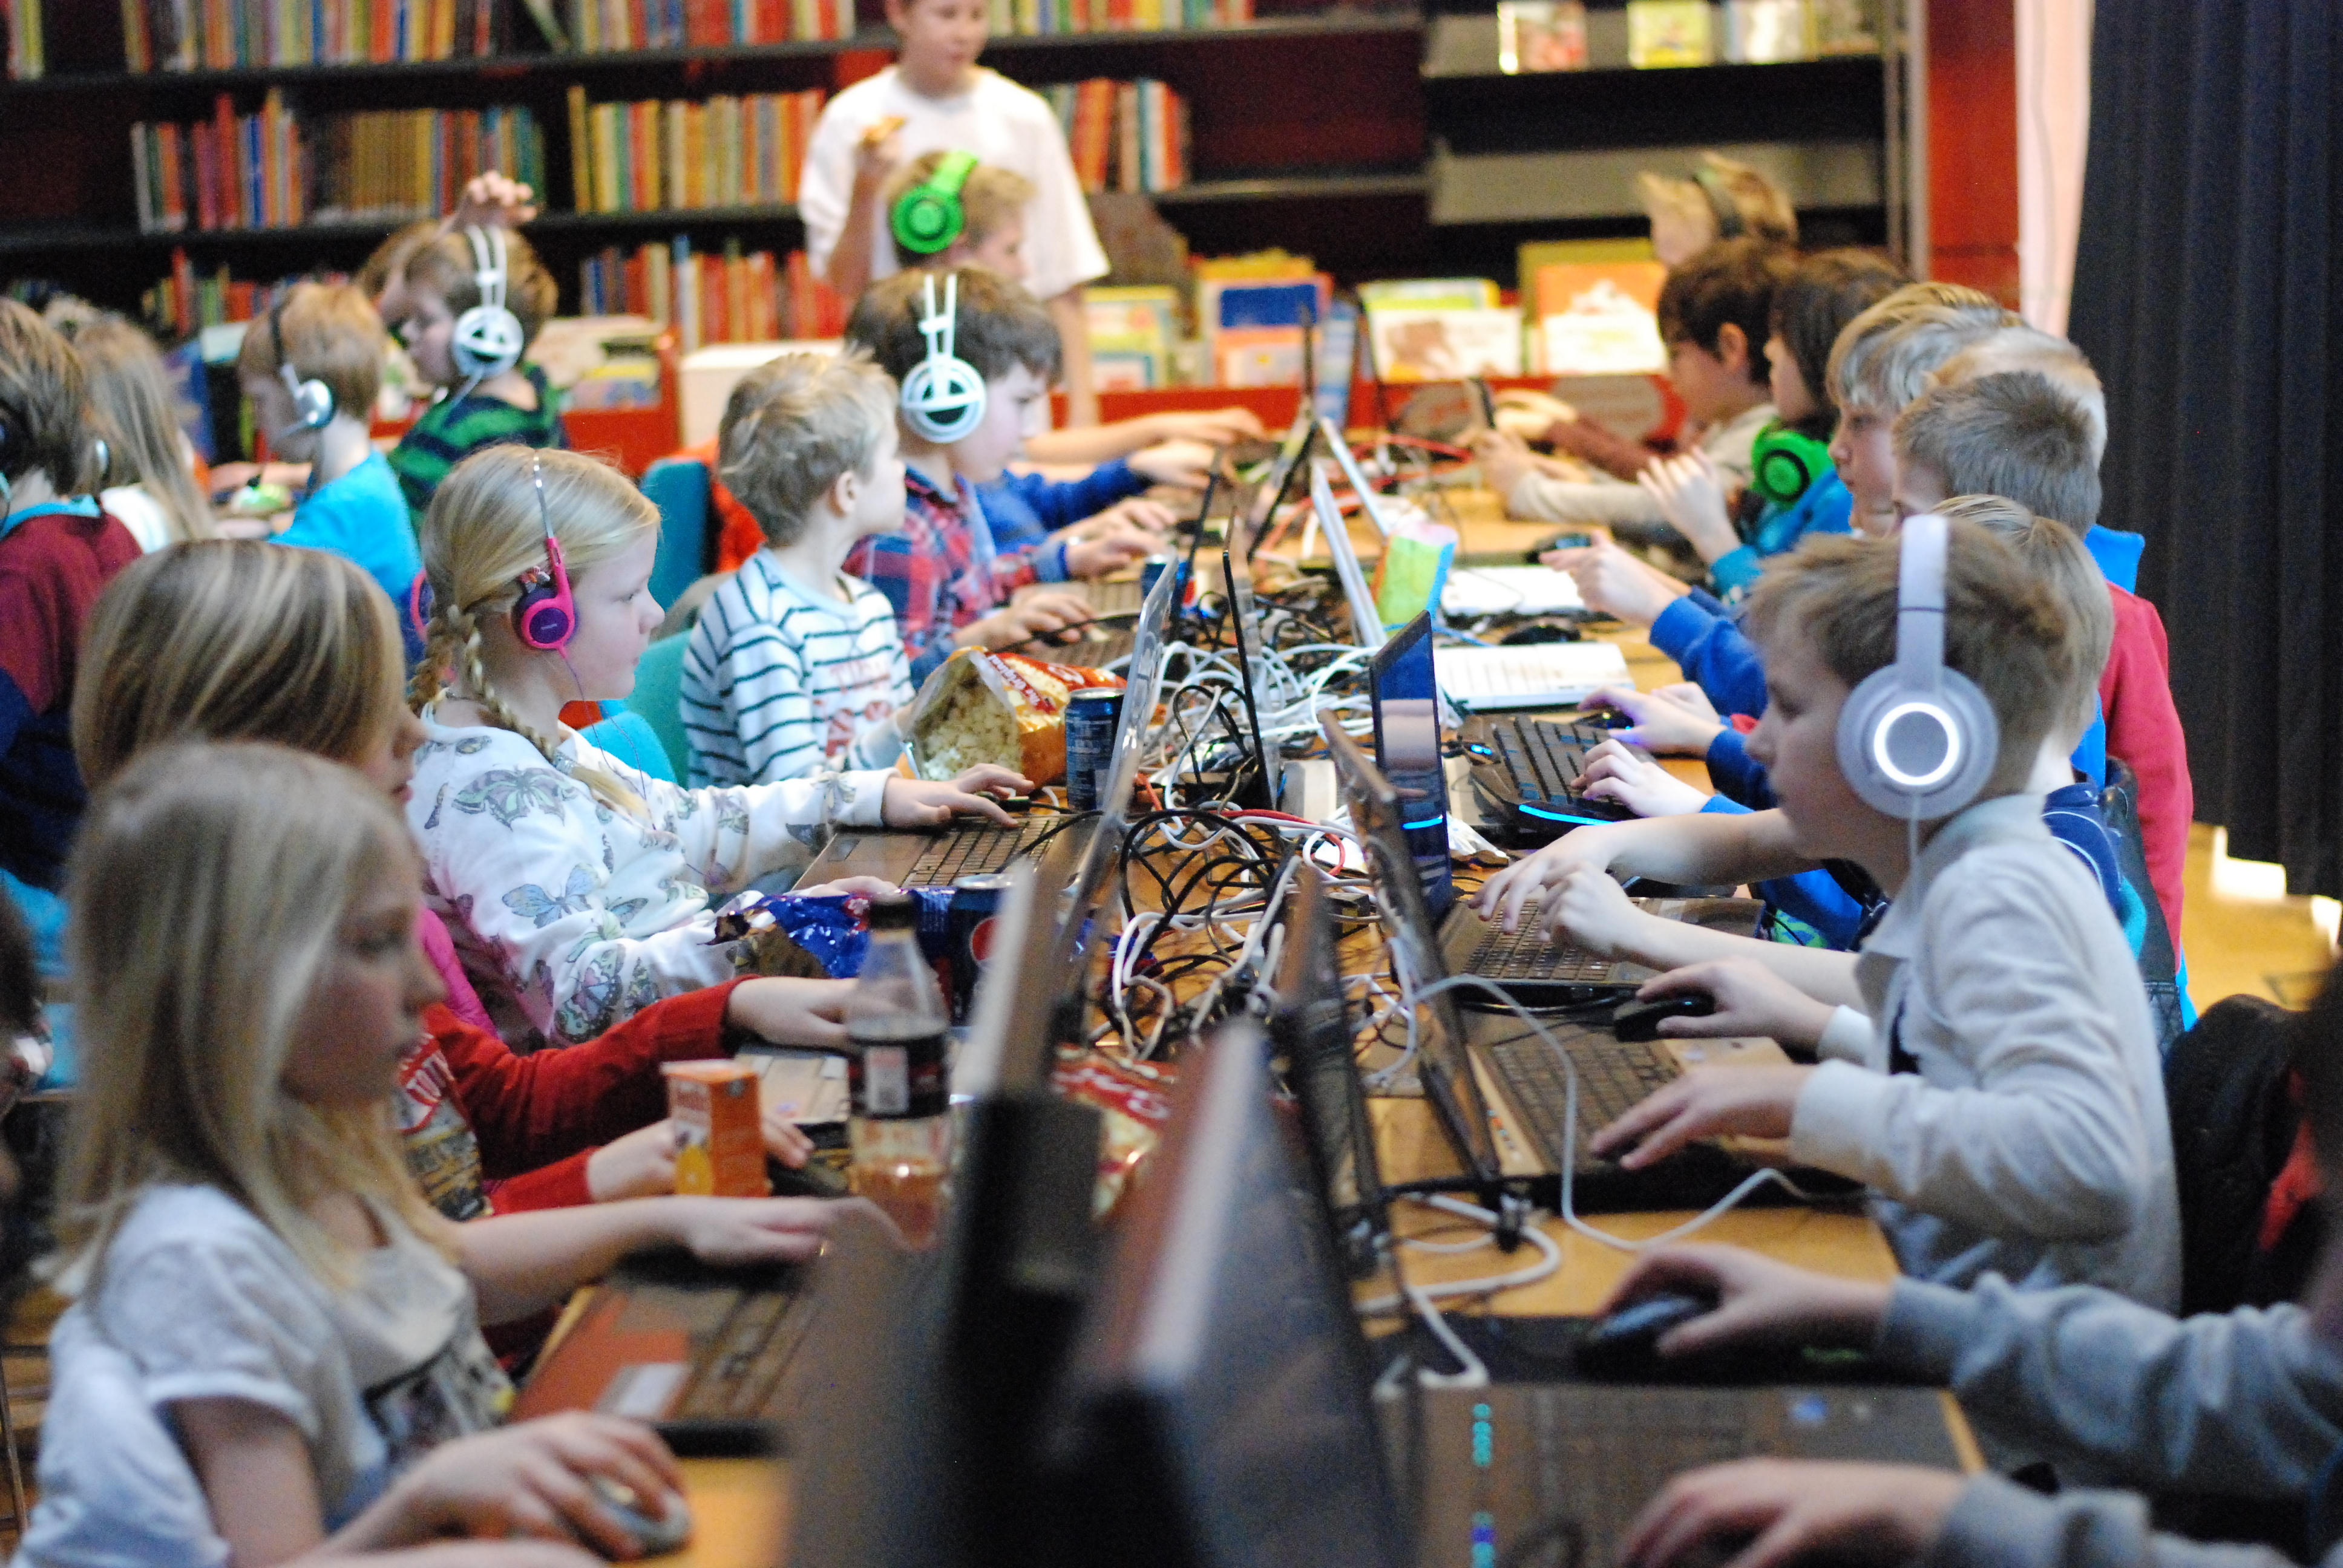
\includegraphics[height=1.2\paperheight]{Pictures/kids-programming}%
  };
  \end{tikzpicture}%
  \end{figure}%
  \end{frame}%


\begin{frame}[plain]
  \begin{figure}
  \centering
  \begin{tikzpicture}[overlay] 
  \node [] at (0.0mm,-5.0mm) {%
  \includegraphics[height=1.2\paperheight]{Pictures/titlepictureGroup}};
  \end{tikzpicture}%
  \end{figure}%
  \end{frame}%

\begin{Slide}{About our Scala students at Lund Univesity}
\begin{itemize}
\item Enrolled at the 5 year program in Computer Science \& Engineering (CSE) at LTH
\item Taking their first programming course 7.5 ECTS credits during their first semester
\item More than 80\% are 19--22 years old
\item Around 15\% are female     
\item 100\% are fluent in, or native, Swedish
\item Around 65\% have programmed before (C\#, Java, Python, Javascript, ...)
\item Very big span of pre-knowledge
\item Increasingly selective admission: 136 accepted out of 1337 applicants (2018)
\end{itemize}
\end{Slide}

\begin{Slide}{History of first languages at Lund University}
First languages for CSE students at LTH:
\begin{table}
\begin{tabular}{l l}
(Algol) & (pre-history using punch cards) \\
 Pascal & 1982, CSE program started\\
 Simula &  1990 \\
 {\color{blue}\textbf{Java}} &  1997 \\
 {\color{red}\textbf{Scala}} &  2016 \\
\end{tabular}
\end{table}

\end{Slide}

\begin{Slide}{The first year of the CSE program since 2016}
\begin{table}
\begin{tabular}{l| p{2.5cm} p{2.5cm} | p{2.5cm} p{2.5cm} }
  Semester & \multicolumn{2}{l}{Fall semester, 30hp } & \multicolumn{2}{|l}{Spring semester, 30hp} \\ \hline
  Period & 1 & 2 & 3 & 4 \\ 
  & \multicolumn{2}{c|}{\tikz{\node [draw, text width=5.22cm, align=center, fill=red!40] {\bf Programming 1 \newline (Scala) 7.5hp};}} 
  & \tikz{\node [draw, text width=2.5cm, align=center, fill=blue!40] {Progr. 2 (Java) 7.5hp };} 
  & \tikz{\node [draw, text width=2.5cm, align=center] {\small Discr. struct. (Closure) 5hp };} 
  \\
  & \tikz{\node [draw, text width=1.5cm, align=center, fill=red!10] {\small Computer intro. 3hp};} 
  & \tikz{\node [draw, text width=2.3cm, align=center] {\small Cognition 4.5hp};} 
  & \multicolumn{2}{c}{\tikz{\node [draw, text width=5.4cm, align=center] {\small Evaluation of software systems  (R) \newline 7hp};}} 
  \\
  & \multicolumn{2}{c|}{\tikz{\node [draw, text width=5.2cm, align=center] {\small Mathematics: \newline Calculus in one variable  \newline 15hp};}} 
  & \tikz{\node [draw, text width=2.5cm, align=center] {\small Physics: photonics 5hp};}
  & \tikz{\node [draw, text width=2.5cm, align=center] {\small Math: linear algebra 6hp};}
  \\
  
\end{tabular}
\end{table}  
{\small A study year is 60 ECTS higher education points (hp) = 40 weeks of full-time studies. }

\end{Slide}

\begin{Slide}{The Java first situation (2015)}
  I took over as course head of the first programming course in 2015 and ran it (almost) as usual with Java first, while in parallell heading the development of the Scala first course material as an open source community project with colleagues and senior students.

  \vspace{0.5em}%
  \begin{minipage}[t]{0.42\textwidth}
      \textbf{Good}:
      \begin{itemize}
        \item Course very popular
        \item Exam results very good:  
        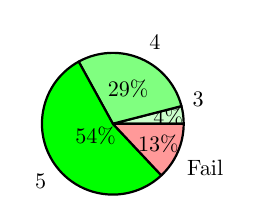
\begin{tikzpicture}[scale=0.3, every node/.style={scale=0.8}]
          \pie [color={green!20, green!50, green, red!40} ]  {4/3, 29/4, 54/5, 13/Fail}
          % inclding W {8/3, 28/4, 48/5, 16/Fail}
        \end{tikzpicture}
      
      \end{itemize}
    \end{minipage}%
    \begin{minipage}[t]{0.6\textwidth}
      \textbf{Bad}:
      \begin{itemize}
        %\item Some not so enthusiastic about Java         
        \item High-performing students not challenged
        \item Poor results in second course
      \end{itemize}   
      
      \pause\vspace{0.5em}=> \textbf{Goals} of introduction Scala first:
      \begin{itemize}
        %\item Some not so enthusiastic about Java         
        \item Increase challenge level for high-performers 
        \item Increase learning outcome for all students
        \item Improve collaboration among students
      \end{itemize}   
      
    \end{minipage}
\end{Slide}

{
\begin{frame}[plain]
  \begin{tabular}{l | l | l | l | l }
   Grade &  Exam results &  &  & \\
   first & second course &  &  & \\
   course& 2015 {\color{blue}\textbf{Java}} first & 2016 {\color{red}\textbf{Scala}} first & 2017 {\color{red}\textbf{Scala}} first & 2018 {\color{red}\textbf{Scala}} first\\

   {\huge 3} & 
    \begin{minipage}{0.15\textwidth}%
      \centering%
      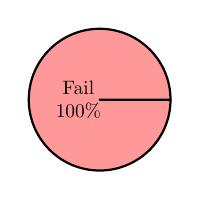
\begin{tikzpicture}[scale=0.3, every node/.style={scale=0.7}]
        \pie [color={green!40, red!40}, text=inside ] {0, 100/Fail}
      \end{tikzpicture}
    \end{minipage}%
     & 
     \begin{minipage}{0.15\textwidth}%
      \centering%
      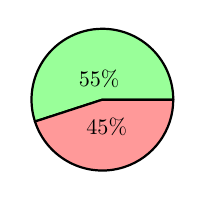
\begin{tikzpicture}[scale=0.3, every node/.style={scale=0.8}]
        \pie [color={green!40, red!40}, text= ] {55/Pass, 45/Fail}
      \end{tikzpicture}
    \end{minipage}%
    & 
    \begin{minipage}{0.15\textwidth}%
     \centering%
     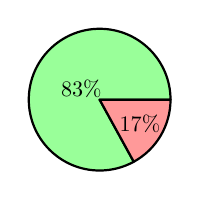
\begin{tikzpicture}[scale=0.3, every node/.style={scale=0.8}]
       \pie [color={green!40, red!40}, text= ] {83/Pass, 17/Fail}
     \end{tikzpicture}
   \end{minipage}%
   & 
   \begin{minipage}{0.15\textwidth}%
    \centering%
    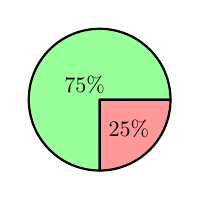
\begin{tikzpicture}[scale=0.3, every node/.style={scale=0.8}]
      \pie [color={green!40, red!40}, text= ] {75/Pass, 25/Fail}
    \end{tikzpicture}
  \end{minipage}%
  \\

     {\huge 4} & 
     \begin{minipage}{0.15\textwidth}%
       \centering%
       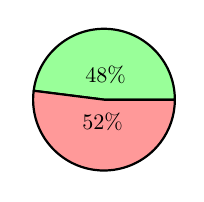
\begin{tikzpicture}[scale=0.3, every node/.style={scale=0.8}]
         \pie [color={green!40, red!40}, text= ] {48/Pass, 52/Fail}
       \end{tikzpicture}
     \end{minipage}%
      & 
      \begin{minipage}{0.15\textwidth}%
       \centering%
       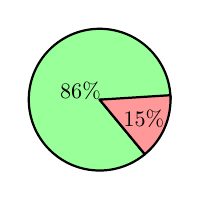
\begin{tikzpicture}[scale=0.3, every node/.style={scale=0.8}]
         \pie [color={green!40, red!40}, text= ] {86/Pass, 15/Fail}
       \end{tikzpicture}
     \end{minipage}%
     & 
     \begin{minipage}{0.15\textwidth}%
      \centering%
      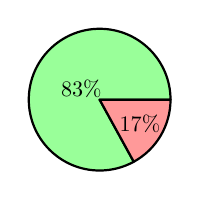
\begin{tikzpicture}[scale=0.3, every node/.style={scale=0.8}]
        \pie [color={green!40, red!40}, text= ] {83/Pass, 17/Fail}
      \end{tikzpicture}
    \end{minipage}%
    & 
    \begin{minipage}{0.15\textwidth}%
     \centering%
     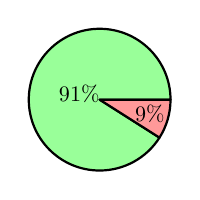
\begin{tikzpicture}[scale=0.3, every node/.style={scale=0.8}]
       \pie [color={green!40, red!40}, text= ] {91/Pass, 9/Fail}
     \end{tikzpicture}
   \end{minipage}%
     \\

      {\huge 5} & 
      \begin{minipage}{0.15\textwidth}%
        \centering%
        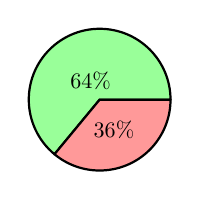
\begin{tikzpicture}[scale=0.3, every node/.style={scale=0.8}]
          \pie [color={green!40, red!40}, text= ] {64/Pass, 36/Fail}
        \end{tikzpicture}
      \end{minipage}%
       & 
       \begin{minipage}{0.15\textwidth}%
        \centering%
        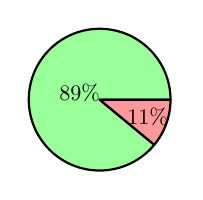
\begin{tikzpicture}[scale=0.3, every node/.style={scale=0.8}]
          \pie [color={green!40, red!40}, text= ] {89/Pass, 11/Fail}
        \end{tikzpicture}
      \end{minipage}%
      & 
      \begin{minipage}{0.15\textwidth}%
       \centering%
       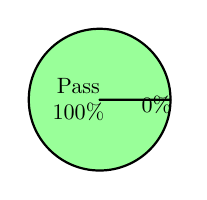
\begin{tikzpicture}[scale=0.3, every node/.style={scale=0.8}]
         \pie [color={green!40, red!40}, text=inside ] {100/Pass, 0/}
       \end{tikzpicture}
     \end{minipage}%
     & 
     \begin{minipage}{0.15\textwidth}%
      \centering%
      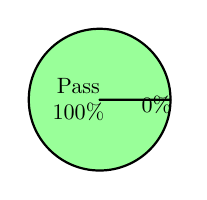
\begin{tikzpicture}[scale=0.3, every node/.style={scale=0.8}]
        \pie [color={green!40, red!40}, text=inside ] {100/Pass, 0/}
      \end{tikzpicture}
    \end{minipage}%
       \\

    \end{tabular}
\end{frame}
}

\begin{Slide}{Scala first -- a big success! \texttt{~:)}}
\begin{itemize}
  \item Exam results in second course much better: increased learning outcome
  \item Course evaluations are still very positive: increased student engagement
  \item All students are challenged, independent of pre-knowledge
  \item Students find Scala interesting and novel
  \item Exam results: \\\vspace{0.5em} 
  \begin{tabular}{l l l}
  2016 & 2017 & 2018 \\
  \begin{minipage}{0.27\textwidth}%
    \centering%
    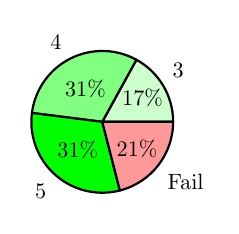
\begin{tikzpicture}[scale=0.3, every node/.style={scale=0.8}]
      \pie [color={green!20, green!50, green, red!40} ]  {17/3, 31/4, 31/5, 21/Fail}
    \end{tikzpicture}
\end{minipage}%
  & 
  \begin{minipage}{0.27\textwidth}%
   \centering%
   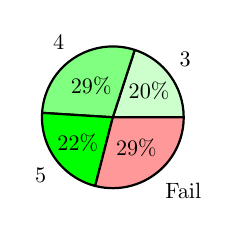
\begin{tikzpicture}[scale=0.3, every node/.style={scale=0.8}]
    \pie [color={green!20, green!50, green, red!40} ]  {20/3, 29/4, 22/5, 29/Fail}
  \end{tikzpicture}
\end{minipage}%
 & 
 \begin{minipage}{0.27\textwidth}%
  \centering%
  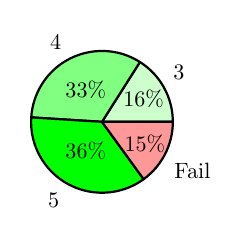
\begin{tikzpicture}[scale=0.3, every node/.style={scale=0.8}]
    \pie [color={green!20, green!50, green, red!40} ]  {16/3, 33/4, 36/5, 15/Fail}
  \end{tikzpicture}
\end{minipage}%
   \\

  \end{tabular}
\end{itemize}

\end{Slide}

% \begin{Slide}{Why not Python first?}
%   My hypotheses based on some experience (but no systematic empiricism):
% \begin{itemize}
%   \item Dynamic typing means less help in finding bugs -> risk of giving up when stuck
%   \item Non-explicit types in function defs is less efficient when learning abstract thinking
%   \item Indentation syntax with silent begin--end makes nested blocks obscure to beginners
%   \item No explicit variable declaration can lead to very hard bugs also for non-beginners 
%   \item Not excellent at object orientation
%   \item Not excellent at functional programming
% \end{itemize}  
% \end{Slide}

\begin{Slide}{Why Scala first?}
  My hypotheses supported by my experience since 2011 (but no systematic empiricism):
  \begin{itemize}
  \item Easy for beginners and interesting for non-beginners (depending how you teach...)
  \item Regular semantics is easier for beginners; e.g. value types are real objects
  \item Concise (but not too concise), expressive: do interesting things with small programs
  \item Powerful, simple-to-use standard library: do interesting things with small programs
  \item Static typing help finding bugs: the compiler is your friend
  \item Interactive learning in the Scala REPL: understand expressions step by step
  %\item Rich semantics: can demonstrate many computer science concepts
  \item Modern, evolving language: exciting for students and teachers
  %\item Free, open source language and tools: no vendor lock-in (cf. .net, Swift)
  \item Multi-paradigm: excellent for mixing imperative, object-oriented, functional
  \end{itemize}  
\end{Slide}


\begin{Slide}{Teaching benefits of a multi-paradigm language}
\begin{minipage}{0.2\textwidth}
  \includegraphics[height=0.52\textheight]{Pictures/marton}\\
  {\small Marton \& Tsui \newline (2004)}
\end{minipage}%
\begin{minipage}{0.85\textwidth}
  \begin{itemize}
    \item Learning is the process of being capable of \textit{doing} something
    \item Learners construct a language by discerning parts and wholes % that are experienced in context   
    \item Patterns of variation:
    \begin{itemize}
      \item \textbf{Contrast}: to experience something, you need to experience something else to compare with    
      \item \textbf{Generalisation}: to understand a concept you need to be able to abstract from irrelevant features    
      \item \textbf{Separation}: to experience a certain aspect of something you need to vary that aspect while other aspects remain invariant    
      \item \textbf{Fusion}: to be capable of doing something advanced you need to experience several critical aspects at the same time    
    \end{itemize}
  \end{itemize}
\end{minipage}

\vspace{1em} Scala enables contrasting, generalisation, separation and fusion across paradigms.

\end{Slide}

\Section{How did we implement Scala first?}

\begin{Slide}{Pedagogical ideas behind course design}
  \begin{minipage}{0.3\textwidth}
    \includegraphics[height=0.6\textheight]{Pictures/brown}\\
    Brown et al. (2014)
  \end{minipage}%
  \begin{minipage}{0.7\textwidth}
    A great summary of research on effective learning strategies:
    \begin{itemize}
      \item How learning occurs: encoding, consolidation, retrieval
      \item Low-stake self testing to retrieve what you learned and identify missing pieces
      \item Deliberate practice: spaced out \& interleaved
      \item Use reflection \& elaboration as you retrieve
      \item Easier isn't better: embrace desirable difficulties
      \item How effort helps: reconsolidation, creating mental models, broaden mastery, foster conceptual learning, improve versatility, prime your mind for learning 
      \item Dismissed myths: errorless learning, learning styles
    \end{itemize}
  \end{minipage}
  
  \end{Slide}

\begin{Slide}{A typical study week}
  Resources for 135 students: 1 lecturer (me), 14 teaching assistants (older students), 
\begin{table}\centering
  \begin{tabular}{l | l |l l | l}
  Mon & Tue & Wed & Thu & Fri \\ \hline
  Lecture (2h) & Lecture (2h) & \multicolumn{2}{c|}{Workshop (2h)} & Lab session (2h) \\ \hline
  \end{tabular}
\end{table}
  \begin{itemize}
    \item Workshops and labs in school computer rooms with Ubuntu and preinstalled tools. 
    \item Workshops have 1 teaching assistant per 12 students. 
    \item 7 workshop time slots (2h) in 2 rooms in parallell.
    \item 2 lab time slots (2h) in 6 rooms in parallell.
    \item If there is space left in room you can attend several workshops.
    \item Computer rooms are available to students 24/7 when no teaching is scheduled.
  \end{itemize}

\vfill Link to schedule: \url{http://cs.lth.se/pgk/schema/}
\end{Slide}  

\begin{Slide}{Progression}
  \fontsize{7}{9}\selectfont
  \begin{tabular}{l|l|l|l}
    \textit{Week} & \textit{Module} & \textit{Workshop} & \textit{Lab} \\ \hline \hline
    W01 & Introduction & expressions & kojo \\
    W02 & Programs & programs & -- \\
    W03 & Functions & functions & irritext \\
    W04 & Objects & objects & blockmole \\
    W05 & Classes & classes & blockbattle \\
    W06 & Sequences & sequences & shuffle \\
    W07 & Set, Map & lookup & words \\
        & Diagnostic test & -- & -- \\
    W08 & Matrices & matrices & life \\
    W09 & Inheritance & inheritance & snake \\
    W10 & Patterns, exceptions & patterns & tabular \\
    W11 & Scala vs Java & scala-java & javatext \\
    W12 & Sorting & sort & -- \\
    W13--W14 & Exam prep., projekt & examprep & Projekt \\
        & Written exam & -- & -- \\
    \end{tabular}  
\end{Slide}

\begin{Slide}{The first three weeks are playful}
  
  \begin{itemize}
    \item Computing course in parallel with intro to terminal on school computers (Ubuntu)
    \item Student's traditional freshman games and festivities in parallell
    \item Week 1: Easy intro to programming is using REPL and Kojo with turtle graphics%: \url{http://www.kogics.net/kojo-download}: \\ Working with expressions in REPL and control flow principles (SARA) in Kojo: 
    \begin{itemize}
      \item \textbf{S}equence (statements)
      \item \textbf{A}lternative (if statements)
      \item \textbf{R}epetition (repeat construct without loop variable)
      \item \textbf{A}bstraction (simple functions)   
    \end{itemize}
    \item Week 2: small readln println programs \\ compile in terminal with \code|scalac|, run with \code|scala|
    \item Week 3: create a lagom irritating terminal text game at your challenge level \\ compile \& run with \code|sbt ~run| , you should divide your game into several functions   
  \end{itemize}
\footnotesize{https://en.wikipedia.org/wiki/Lagom}
\end{Slide}  


  


\begin{Slide}{Continuous examination: Lab sessions}
  
\end{Slide}  

\begin{Slide}{Mid term diagnostic test: early warning}
  
\end{Slide}  


\begin{Slide}{Final exam: securing the learning outcome}
  
\end{Slide}  


\Section{What did we learn?}

\begin{Slide}{Designing a progression with Scala first}
\begin{itemize}
  \item Start with Expressions and simple functions first, and then small but complete programs with imperative statements \& procedures 
  \item Objects are introduced as modules to create name space
  \item Classes are introduced as several instances are needed
  \item Case classes introduced together with general classes: \\
   contrast immutable data and instances with mutable state
  \item Inheritance introduced late, except for enumerations
\end{itemize}
\end{Slide}  


\begin{Slide}{}
  
\end{Slide}  

\begin{Slide}{Functions for abstraction, modules for name}
  
\end{Slide}  


\begin{Slide}{Balance between object-oriented and functional}
  
\end{Slide}  


\Section{The road ahead}


\EndSlide

\end{document}